\documentclass{AeroStructure-ERJohnson}
\input crosslink.tex

%\usepackage{showframe}
\def\ShowFrameLinethickness{0.125pt}

\def\harp#1{\smash{\mathord{\buildrel{\lower3pt\hbox{$\scriptscriptstyle\rightharpoonup$}}\over{#1}}}}

\myexternaldocument{App_4P}
\myexternaldocument{Ch01_4P}
\myexternaldocument{Ch02_4P}
\myexternaldocument{Ch03_4P}
\myexternaldocument{Ch04_4P}
\myexternaldocument{Ch05_4P}
\myexternaldocument{Ch06_4P}
\myexternaldocument{Ch07_4P}
\myexternaldocument{Ch08_4P}
\myexternaldocument{Ch09_4P}
%\myexternaldocument{Ch10_4P}
\myexternaldocument{Ch11_4P}
\myexternaldocument{Ch12_4P}
\myexternaldocument{Ch13_4P}
\myexternaldocument{Ch14_4P}
\myexternaldocument{Ch15_4P}
\myexternaldocument{Ch16_4P}
\myexternaldocument{Ch17_4P}
\myexternaldocument{Ch18_4P}


\begin{document}


\mainmatter

%\hbox{~}\clearpage
\setcounter{page}{265}

\setcounter{chapter}{9}

\chapter{Structural stability of discrete conservative systems}\label{ch10}

Structures subject to compression fail in differently than those subject to tension. For some ductile metals that are short and thick, compression failure is associated with a shear mechanism with a fracture plane inclined with respect to the axis of the compressive load. Other ductile metals may not fracture in compression but crush during plastic deformation. Long and thin compression members fail by buckling in which the member responds by displacing sideways with respect to the direction of the compressive load. Buckling is characterized by
\begin{itemize}
  \item failure due to excessive displacements (loss of structural stiffness), and/or
  \item loss of stability of an equilibrium configuration
\end{itemize}

\textit{Stability of equilibrium} means that the response of the structure due to a small disturbance from its equilibrium configuration remains small; the smaller the disturbance the smaller the resulting magnitude of the displacement in the response. If a small disturbance causes large displacement, perhaps even theoretically infinite, then the equilibrium state is unstable. Practical structures in engineering are stable at no load. Now consider increasing the load slowly. We are interested in the value of the load, called the \textit{critical load}, at which buckling occurs. That is, we are interested when a sequence of stable equilibrium states as a function of the load, one state for each value of the load, ceases to be stable.

In this chapter structural stability phenomena, concepts, and methods are presented by analyzing discrete systems composed of rigid bars and springs. Stability of discrete systems are also presented by Simitses (1976), and in a monograph by Huseyin (1975). The latter author presents a general non-linear theory of elastic stability of discrete systems. Continuum analyses for the buckling of columns and plates are discussed in the next chapter.

\section{Model A: stable symmetric bifurcation buckling}\label{sec10.1}


This model is shown in figure~\ref{fig10.1} and it has one coordinate $\theta, -\pi < \theta < \pi$, to describe the configuration of the model under the \textit{deadweight load P}. (An external load independent of its corresponding displacement.) The model consists of a rigid rod of length \textit{L}, connected by smooth hinge to a rigid base. The rod can rotate about the hinge, but it is restrained by a linear elastic torsional spring of stiffness \textit{K} (dimensional units of F-L/ radian). The restoring moment of the spring acting on the bar is zero at $\theta = 0$. Neglect the weight of the rod with respect\vadjust{\vspace*{10pt}\pagebreak} to the applied load \textit{P}. From the free body diagram of the rod shown in figure~\ref{fig10.1}, the equation of motion for rotation about the fixed hinge is
\begin{equation}\label{eq10.1}
P L \sin \theta-K \theta=I_{0} \frac{d^{2} \theta}{d t^{2}} \quad \theta=\theta(t) \quad t>0
\end{equation}
where ${I_0}$ is the moment of inertia of the rod about the fixed point and $t$ is time.

\processfigure[t]{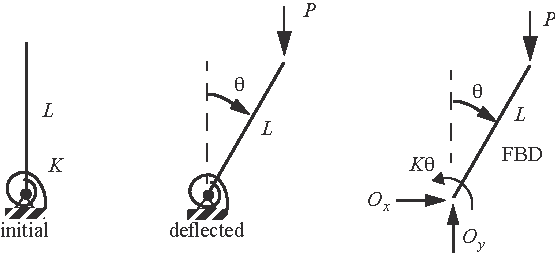
\includegraphics{Figure_10-1.pdf}}{\caption{One degree-of-freedom structural model.\label{fig10.1}}}




\subsection{Equilibrium method}\label{sec10.1.1}

This method is also known as the classical method or bifurcation method. Consider equilibrium states under the static, downward load \textit{P} which are characterized by the angle $\theta$ being independent of time $t$. Hence, the inertia term in eq.~(\ref{eq10.1}) vanishes and we have
\begin{align}\label{eq10.2}
P L \sin \theta-K \theta=0 \quad|\theta|<\pi.
\end{align}
One solution to eq.~(\ref{eq10.2}) is
\begin{align}\label{eq10.3}
p 1: \theta=0 \text { for any } {P}.
\end{align}
Equilibrium path (\ref{eq10.3}) is called the trivial equilibrium configuration. The equilibrium method is characterized by the question
\begin{quote}
\textit{What are the values of the load for which the perfect system admits non-trivial equilibrium configurations? (Ziegler, 1968)}
\end{quote}

A second solution of eq.~(\ref{eq10.2}) is
\begin{equation}\label{eq10.4}
p 2: P=\left(\frac{K}{L}\right) \frac{\theta}{\sin \theta}
\end{equation}
Recall from the calculus using l'H\^{o}pital's rule that the limit of the indeterminate form $\theta /(\sin \theta)$ as $\theta \rightarrow 0$ is one. The two equilibrium paths are plotted in the load-deflection diagram shown in figure~\ref{fig10.2}. Equilibrium path \textit{p2} is called the secondary path and we note it is symmetric about $\theta = 0$. For $P<K / L$ there is only one equilibrium position: $\theta=0$ on the primary path \textit{p1}. For $P>K / L$ there are three equilibrium positions: $\theta=0$ on path \textit{p1}, and two on the secondary path \textit{p2}.

The two equilibrium paths intersect at $(\theta,\;\textit{P}) = (0,\;\textit{K/L})$. This intersection of the two paths is called a \textbf{bifurcation point}, and represents the equilibrium state or position common to two separate equilibrium paths. At no load the rod is vertical and this corresponds to the origin in the load-deflection diagram. As the load \textit{P} is slowly increased from zero the rod remains vertical ($\theta = 0$), and at ${P = K/L}$ adjacent equilibrium states exists on the secondary path\vspace*{10pt}.

\begin{wrapfigure}[15]{R}{168pt}
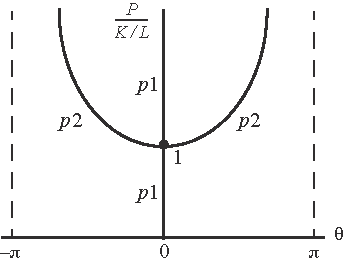
\includegraphics{Figure_10-2.pdf}
\caption{Equilibrium paths\label{fig10.2}}
\end{wrapfigure}

The existence of adjacent equilibrium states in the vicinity of the primary equilibrium path has been noted by investigators of structural stability as the onset of buckling. Hence, buckling is characterized by the bifurcation point on the load-deflection diagram. For this reason, the term bifurcation buckling is used to describe this condition. As we will show later, the rod will not remain vertical for loads \textit{P > K/L} if there are infinitesimal disturbances present (there always are), but will rotate either to the left or right depending on type of infinitesimal disturbance. We note that the magnitude of the angle $\theta$ becomes large as the load is increased from \textit{K/L} on the secondary path. The load at the bifurcation point is called the critical load and is denoted as $P_{{cr}}$. Thus,\vspace*{-3pt}
\begin{align}\label{eq10.5}
P_{c r}=K / L.
\end{align}

\vspace*{-6pt}

\subsubsection{Small $\boldsymbol{\theta}$ analysis} Consider the small angles of rotation such that $\sin \theta \approx \theta$ for $\theta$ measured in radians.~Equili\-brium eq.~(\ref{eq10.2}) becomes\vspace*{-6pt}
\begin{align}\label{eq10.6}
P L \theta-K \theta=0.
\end{align}
The solutions of this equation (\ref{eq10.6}) are\vspace*{-6pt}
\begin{align}\label{eq10.7}
p 1^{\prime}: \quad \theta=0\ \text{for any}\ P,\ \text{and}\\
\label{eq10.8}
p 2^{\prime}: \quad P=K / L\ \text{for any small}\ \theta.
\end{align}
\begin{wrapfigure}[10]{r}{90pt}
\vspace{-19pt}
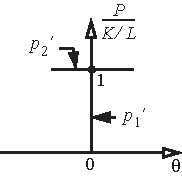
\includegraphics{Figure_10-3.pdf}
\caption{Small $\theta$ analysis.\label{fig10.3}}
\end{wrapfigure}
These solutions are shown in the load-deflection plane in figure~\ref{fig10.3}. The equilibrium path $p 1^{\prime}$ coincides with path \textit{p1}, but path $p 2^{\prime}$ is not a good approximation to path \textit{p2} unless $\theta$ is very small. However, the bifurcation point is the same as obtained in the large $\theta$-analysis. Hence, the critical load from the small $\theta$-analysis is the same as obtained in eq.~(\ref{eq10.5}) from the large $\theta$-analysis.%\vspace*{-6pt}




\subsection{Kinetic method}\label{sec10.1.2}

The kinetic method, or the vibration method, is based on the definition of stability of equilibrium. The vibration method is characterized by the question
\begin{quote}
\textit{What is the value of the load for which the most general free motion of the perfect system in the equilibrium position ceases to be bounded? (Ziegler, 1968)}
\end{quote}
\begin{wrapfigure}[16]{r}{74pt}
\vspace{10pt}
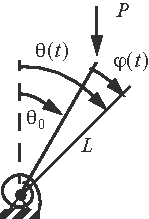
\includegraphics{Figure_10-4.pdf}
\caption{Rotations in the stability analysis.\label{fig10.4}}
\end{wrapfigure}

Let the rotation angle\vspace*{-6pt}
\begin{align}\label{eq10.9}
\theta(t)=\theta_{0}+\varphi(t),
\end{align}
where $\theta_{0}$ is independent of time and satisfies the equilibrium eq.~(\ref{eq10.2}); i.e.,
\begin{align}\label{eq10.10}
P L \sin \theta_{0}-K \theta_{0}=0.
\end{align}
\noindent Consider the additional rotation angle $\varphi(t)$ to be small in magnitude but a function of time. Thus, we are considering small oscillations about an equilibrium state $\left(P, \theta_{0}\right)$ as shown in figure~\ref{fig10.4}. Substitute eq.~(\ref{eq10.9}) for $\theta(t)$ in the equation of motion, eq.~(\ref{eq10.1}), to get
\begin{align}\label{eq10.11}
I_{0} \ddot{\varphi}+K(\theta_{0}+\varphi)-P L \sin \left(\theta_{0}+\varphi\right)=0,
\end{align}
where the dots denote derivatives with respect to time \Big(e.g., $\ddot{\varphi}=\frac{d^{2} \varphi}{d t^{2}}$\Big). Using the trigonometric identity for the sine of the sum of two angles, and performing some minor rearrangements, equation (\ref{eq10.11}) becomes\pagebreak
\begin{align}\label{eq10.12}
I_{0} \ddot{\varphi}+K \theta_{0}+K \varphi-P L\left[\sin \theta_{0} \cos \varphi+\cos \theta_{0} \sin \varphi\right]=0.
\end{align}
Now expand the trigonometric functions of angle $\varphi$ in a Taylor Series about $\varphi=0$ to get
\begin{align}\label{eq10.13}
I_{0} \ddot{\varphi}+K \theta_{0}+K \varphi-P L \sin \theta_{0}\left[1-\frac{1}{2} \varphi^{2}+O(\varphi^{4})\right]-P L \cos \theta_{0}\left[\varphi-\frac{1}{6} \varphi^{3}+O(\varphi^{5})\right]=0,
\end{align}
in which $O\left(\varphi^{n}\right)$ means terms of order $\varphi^{n}$ and higher. Arrange eq.~(\ref{eq10.13}) in powers of $\varphi$ to get
\begin{align}\label{eq10.14}
I_{0} \ddot{\varphi}+\underbrace{\left(K \theta_{0}-P L \sin \theta_{0}\right)}_{=0}+\left(K-P L \cos \theta_{0}\right) \varphi+\left(\frac{P L}{2} \sin \theta_{0}\right) \varphi^{2}+\left(\frac{P L}{6} \cos \theta_{0}\right) \varphi^{3}+O(\varphi^{4})=0.
\end{align}
Note that ``coefficient'' of the term $\varphi^{0}$ vanishes because of the equilibrium condition given by eq.~(\ref{eq10.10}).

For very small additional rotation angles $\varphi(t)$ about the equilibrium configuration, eq.~(\ref{eq10.14}) is approximated~by\vspace*{-6pt}
\begin{align}\label{eq10.15}
I_{0} \ddot{\varphi}+\left(K-P L \cos \theta_{0}\right) \varphi=0 \quad \text { or } \quad \ddot{\varphi}+\omega^{2} \varphi=0,
\end{align}
where
\begin{align}\label{eq10.16}
\omega^{2}=\left(K-P L \cos \theta_{0}\right) / I_{0}.
\end{align}
The solution of the second order differential equation (\ref{eq10.15}) for $\omega^{2}>0$ is
\begin{align}\label{eq10.17}
\varphi(t)=A_{1} \sin (\omega t)+A_{2} \cos (\omega t) \quad \omega^{2}>0,
\end{align}
in which constants $A_{1}$ and $A_{2}$ are determined by initial conditions for $\varphi(0)$ and $\dot{\varphi}(0)$. The solution given by eq.~(\ref{eq10.17}) is a harmonic oscillation about the equilibrium configuration and $\omega$ is interpreted as the natural frequency in radians per second. Initial conditions $\varphi(0)$ and $\dot{\varphi}(0)$ are considered to be very small to simulate an arbitrary infinitesimal disturbance. The smaller the initial disturbance, the smaller the maximum amplitude of the oscillation in $\varphi$. Thus, $\omega^{2}>0$ is a condition for a stable equilibrium configuration with respect to infinitesimal disturbances.

The solution of the second order differential equation, eq.~(\ref{eq10.15}), for $\omega^{2}<0$ is
\begin{align}\label{eq10.18}
\varphi(t)=A_{1} e^{\bar{\omega} t}+A_{2} e^{-\bar{\omega} t} \quad \bar{\omega}^{2}=-\omega^{2}=-\left(K-P L \cos \theta_{0}\right) / I_{0}.
\end{align}
For arbitrary initial conditions, the term with the positive exponent in the dominates the solution. This corresponds to large values of the $\varphi$ no matter how small the initial disturbance. Hence, $\omega^{2}<0$ is a condition of unstable equilibrium configuration with respect to infinitesimal disturbances. The kinetic method for model A leads to the following criterion.\enlargethispage{0.6\baselineskip}

\begin{table}[!h]
\begin{center}
\vspace*{-3pt}
\begin{tabular}{@{}l|l@{}}
%\toprule
\multicolumn{2}{@{}l}{\textbf{Dynamic criterion for stability of an equilibrium state}}\\
\toprule\\[-15.5pt]
 \\[-6pt]
\text{The equilibrium state is stable if} & $\omega^{2}>0$\\
\text{The equilibrium state is critical if} & $\omega^{2}=0$\\
\text{The equilibrium state is unstable if} & $\omega^{2}<0$\\[-9pt]
 \\[-3.5pt]
\botrule
\end{tabular}
\vspace*{-3pt}
\end{center}
\end{table}

On the primary equilibrium path \textit{p1} given by eq.~(\ref{eq10.3}), we have from eq.~(\ref{eq10.16}) that
\begin{align}\label{eq10.19}
\omega^{2}=(K-P L) / I_{0} \quad \text { on } p 1.
\end{align}

\begin{wrapfigure}[13]{r}{129pt}
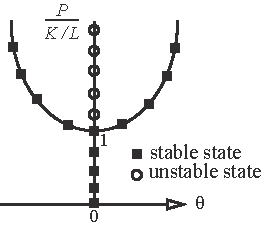
\includegraphics{Figure_10-5.pdf}
\caption{Stability of the equilibrium states for model~A.\label{fig10.5}}
\end{wrapfigure}



\noindent Thus, equilibrium configurations are stable if $P<K / L$, critical if $P=K / L$, and unstable if $P>K / L$. The primary equilibrium path ceases to be stable at $P=P_{c r}$, and $P_{c r}$ is the buckling load. On the secondary path (\ref{eq10.4}) $\omega^{2}=\left[K\left(1-\theta_{0} \cot \theta_{0}\right)\right] / I_{0}$, and $\omega^{2} \geq 0$ for $0<\left|\theta_{0}\right|<\pi$, Thus, the equilibrium configuration on the secondary path is critical at $\theta_{0}=0$, and the equilibrium configurations for $0<\left|\theta_{0}\right|<\pi$ are stable. Retaining the first non-zero term in the expansion of the differential equation of motion (\ref{eq10.13}) at the bifurcation point $\left(\theta_{0},\; P\right)=(0,\; K / L)$ we get
\begin{align}\label{eq10.20}
\ddot{\varphi}+\left(\frac{K}{6 I_{0}}\right) \varphi^{3}=0.
\end{align}
Differential equation of motion (\ref{eq10.20}) is nonlinear. Since coefficient $K /\left(6 I_{0}\right)>0$, its solution is a nonlinear oscillation about the bifurcation point for small initial disturbances (Simitses, 1976). Hence, equilibrium at the bifurcation point is stable. The stability of the equilibrium states for model A are shown in figure~\ref{fig10.5}.


\subsection{Energy method}\label{sec10.1.3}

\subsubsection{Theorem.} A conservative mechanical system is in a configuration of stable equilibrium if, and only if, the value of the potential energy is a relative minimum, otherwise it is unstable.

This method is characterized by the question:

\begin{quote}
\textit{What is the value of the load for which the potential energy of the system in the equilibrium position ceases to be positive definite? (Ziegler, 1968)}
\end{quote}
\begin{wrapfigure}[14]{r}{124pt}
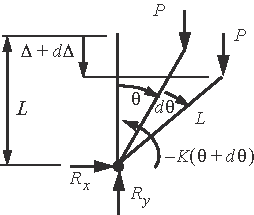
\includegraphics{Figure_10-6.pdf}
\caption{Forces acting on the bar of model A for an increment in its
rotation.\label{fig10.6}}
\end{wrapfigure}

First we have to determine if model A is a conservative mechanical system. The incremental work of the external load and the rotational spring acting on the bar shown in figure~\ref{fig10.6} are given by
\begin{align}\label{eq10.21}
d W_{\mathrm{ext}}=P(\Delta+d \Delta)-P \Delta=P d \Delta \quad d W_{\mathrm{int}}=-[K(\theta+d \theta)-K \theta]=-(K \theta) d \theta.
\end{align}
\noindent
The incremental external work is positive since load \textit{P} and the shortening $\Delta$ act in the same direction, but the incremental work of the spring on the bar opposes the increase in rotation. The shortening is given by
\begin{align}\label{eq10.22}
\Delta=L(1-\cos \theta).
\end{align}
The increment in the shortening with respect to an infinitesimal change in the rotation is
\begin{align}\label{eq10.23}
d \Delta=\frac{d \Delta}{d \theta} d \theta=(L \sin \theta) d \theta.
\end{align}
The incremental external work is $d W_{\mathrm{ext}}=P L \sin \theta d \theta$. Since the load \textit{P} is independent of angle $\theta$ for deadweight loading, we can integrate incremental work expression to get $W_{\mathrm{ext}}=-P L \cos \theta+C$. The constant C is determined if we define $W_{\text {ext}}=0$ when $\theta = 0$. The external work function is
\begin{align}\label{eq10.24}
W_{\text {ext }}=P L(1-\cos \theta).
\end{align}
Note that the work of \textit{P} is independent of path. For example, the value of $W_{\text {ext }}$ is the same if the bar first rotated to $2\theta$ and then rotated back to $\theta$. The expression for the incremental work of the spring acting on the bar is integrated with respect to $\theta$ to get $W_{\text {int}}=-\frac{1}{2} K \theta^{2}+C'$. The constant $C'$ is determined if we define $W_{\text {int }}=0$ at $\theta = 0$. Hence,
\begin{align}\label{eq10.25}
W_{\text {int }}=-K \theta^{2} / 2.
\end{align}
Since the work done by the external load and the spring force are independent of the process of how the final value of $\theta$ is achieved, they are conservative forces. The potential energy is defined as the negative of the work function. The negative sign means that the work done by the spring force against the rotation increases the potential energy while the work done by the force \textit{P} with the rotation decreases the potential energy. Let $U$ denote the potential energy of the spring and let $\Omega$ denote the potential energy of the external load. Then
\begin{align}\label{eq10.26}
U=\frac{1}{2} K \theta^{2} \quad \Omega=-P L(1-\cos \theta).
\end{align}
The total potential energy is denoted by \textit{V}, where
\begin{align}\label{eq10.27}
V(\theta)=U(\theta)+\Omega(\theta)=\frac{1}{2} K \theta^{2}-P L(1-\cos \theta).
\end{align}

\vspace*{-1pc}

Second, we must determine the equilibrium positions and if these correspond to a relative minimum of \textit{V}. A necessary condition for a relative minimum is that \textit{V} is stationary with respect to $\theta$, and this leads to equilibrium. That is,
\begin{align}\label{eq10.28}
\frac{d V}{d \theta}=0=K \theta-P L \sin \theta,
\end{align}
which is the same equation (\ref{eq10.2}) governing equilibrium found from the free body diagram approach. Let $\theta_{0}$ denote the rotation of the bar in equilibrium under load \textit{P}, or $K \theta_{0}-P L \sin \theta_{0}=0$. The Taylor series of the potential energy about the equilibrium position is
\begin{align}\label{eq10.29}
V\left(\theta_{0}+h\right)=V\left(\theta_{0}\right)+V_{1}\left(\theta_{0}\right) h+\frac{1}{2 !} V_{2}\left(\theta_{0}\right) h^{2}+\frac{1}{3 !} V_{3}\left(\theta_{0}\right) h^{3}+\frac{1}{4 !} V_{4}\left(\theta_{0}\right) h^{4}+\ldots,
\end{align}
where
\begin{align}\label{eq10.30}
h=\theta-\theta_{0} \quad V_{1}\left(\theta_{0}\right)=\left.\frac{d V}{d \theta}\right|_{\theta = \theta_{0}} \quad V_{2}\left(\theta_{0}\right)=\left.\frac{d^{2} V}{d \theta^{2}}\right|_{\theta = \theta_{0}} \quad \text { et cetera}.
\end{align}
At equilibrium $V_{1}\left(\theta_{0}\right)=0$.The change in potential energy $\Delta V=V\left(\theta_{0}+d \theta\right)-V\left(\theta_{0}\right)$ is
\begin{align}\label{eq10.31}
\Delta V=\frac{1}{2 !} V_{2}\left(\theta_{0}\right) h^{2}+\frac{1}{3 !} V_{3}\left(\theta_{0}\right) h^{3}+\frac{1}{4 !} V_{4}\left(\theta_{0}\right) h^{4}+\ldots
\end{align}
For infinitesimal changes in $h \neq 0$ from the equilibrium position, the lowest degree term in $h$ dominates the series of $\Delta V$. Consequently, the potential energy is positive definite if $V_{2}\left(\theta_{0}\right)>0$, indefinite if $V_{2}\left(\theta_{0}\right)=0$, and negative definite if $V_{2}\left(\theta_{0}\right)<0$. The second derivative of $V(\theta)$ is
\begin{align}\label{eq10.32}
\frac{d^{2} V}{d \theta^{2}}=K-P L \cos \theta_{0}.
\end{align}
On trivial equilibrium path $\theta_{0}=0$ for any \textit{P}, and the second derivative $\left.\frac{d^{2} V}{d \theta^{2}}\right|_{p 1}=K-P L$. Therefore,
\begin{align}\label{eq10.33}
\left.\frac{d^{2} V}{d \theta^{2}}\right|_{p 1}>0, \text { stable, } P<K /\left.L \quad \frac{d^{2} V}{d \theta^{2}}\right|_{p 1}=0, \text { critical, } P=K /\left.L \quad \frac{d^{2} V}{d \theta^{2}}\right|_{p 1}<0, \text { unstable, } P>K / L.
\end{align}


\begin{wrapfigure}[10]{r}{198pt}
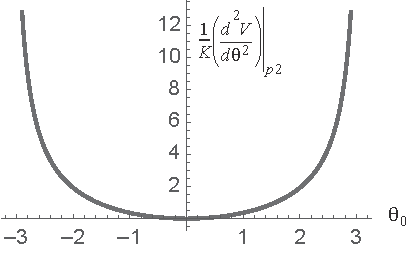
\includegraphics{Figure_10-7.pdf}
\caption{Second derivative of the potential energy on the secondary equilibrium path.\label{fig10.7}}
\end{wrapfigure}
\noindent In answer to the question characterizing the energy method, the potential energy ceases to be positive definite on the primary equilibrium path when $P>K / L$. On the secondary path $P L=K \theta_{0} / \sin \theta_{0}$, and the second derivative of the potential energy is
\begin{align}\label{eq10.34}
\left.\frac{d^{2} V}{d \theta^{2}}\right|_{p 2}=K\left(1-\theta_{0} \cot \theta_{0}\right).
\end{align}
A graph of eq.~(\ref{eq10.34}) is shown in figure~\ref{fig10.7}. Thus,
\begin{align}\label{eq10.35}
&\left.\frac{d^{2} V}{d \theta^{2}}\right|_{p 2} >0, \text { stable, } 0<\left|\theta_{0}\right|<\pi \quad \nonumber\\
&\left.\frac{d^{2} V}{d \theta^{2}}\right|_{p 2}=0 \text {, critical, } P=K /\left.L \quad \frac{d^{2} V}{d \theta^{2}}\right|_{p 2}<0 \text {, unstable, no } \theta \text { of interest}.
\end{align}
These results from the energy method confirm the previous results from the kinetic method. At the bifurcation point $\left(\theta_{0}, P\right)=(0, K / L)$, and the second derivative $V_{2}\left(\theta_{0}\right)=0$. Evaluate the next two terms in the series (\ref{eq10.31}) for $\Delta V$ at the bifurcation point to find
\begin{align}\label{eq10.36}
V_{3}\left(\theta_{0}\right)=\left.\frac{1}{\sin ^{2} \theta_{0}}\left(\theta_{0}-\cos \theta_{0} \sin \theta_{0}\right)\right|_{\theta_{0}\ \rightarrow\ 0}=0 \quad V_{4}\left(\theta_{0}\right)=\left.\frac{2}{\sin ^{3} \theta_{0}}\left(\sin \theta_{0}-\theta_{0} \cos \theta_{0}\right)\right|_{\theta_{0}\ \rightarrow\ 0}=\frac{2}{3}.
\end{align}
The series for $\Delta V$ a the bifurcation point is
\begin{align}\label{eq10.37}
\Delta V=\frac{2}{3} h^{4}+O\left(h^{5}\right).
\end{align}
Hence, $V_{4}(0)>0$, and the bifurcation point $\left(\theta_{0}, P\right)=(0, K / L)$ is stable.




\subsection{Eccentric load}\label{sec10.1.4}
Consider the applied load \textit{P} applied slightly off the center line of the bar by $\delta_{0}$ as shown in figure~\ref{fig10.8}. Moment equilibrium about the fixed pin is

\processfigure[!h]{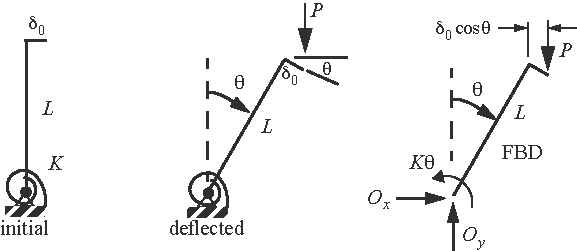
\includegraphics{Figure_10-8.pdf}}{\caption{Model A subject to ecce\-ntric load.\label{fig10.8}}}

\vspace*{-1.8pc}

\begin{align}\label{eq10.38}
P\left(L \sin \theta+\delta_{0} \cos \theta\right)-K \theta=0.
\end{align}
The equilibrium equation (\ref{eq10.38}) solved numerically and the equilibrium paths in the load-deflection plane are shown as dashed lines in figure~\ref{fig10.9}. There are two equilibrium paths: the first one begins from the unloaded state $({P} = 0, \theta = 0)$, and a second complementary path that is not connected to the first path. As the load \textit{P} increases from zero along the first path, the angle $\theta$ increases slowly until \textit{P} is in the vicinity of $P_{\mathrm{cr}}=K / L$. Equilibrium positions on the first path are stable ($\Delta V>0$).

Note the following characteristics.
\begin{itemize}
  \item The deflection for the path beginning from the unloaded state is always the same sign as $\delta_{0}$.
  \item If $\delta_{0}$ is small, the equilibrium path of the imperfect system approaches that of the perfect model as the deflection becomes large.
  \item There is no intersection of two equilibrium paths.
  \item Even if $\delta_{0} \neq 0$ there are three equilibrium states for $P>P_{\mathrm{cr}}$.
  \item There is a minimum load on the complementary path that divides unstable and stable equilibrium states.
\end{itemize}

\processfigure{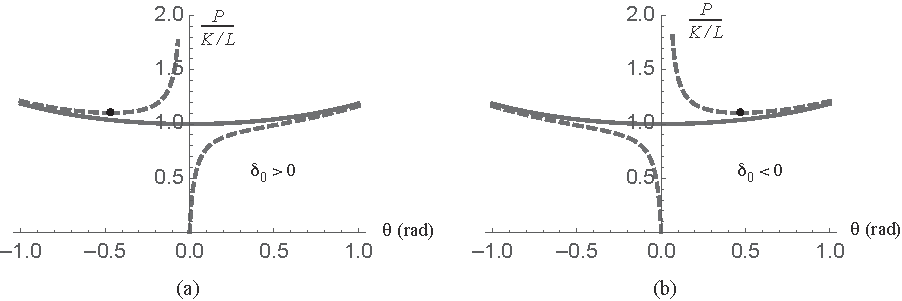
\includegraphics{Figure_10-9.pdf}}{\caption{Load-deflection plots for model A subject to the eccentric load are shown by the dashed
lines for (a) $\boldsymbol{\delta}_{\textbf{0}} \boldsymbol{>} \textbf{0}$ and (b) $\boldsymbol{\delta}_{\textbf{0}} \boldsymbol{<} {\textbf{0}}$.\label{fig10.9}}}



\subsection{Initial angle}\label{sec10.1.5}

When $\textit{P} = 0$, suppose the bar is not vertical but is at an initial angle $\theta=\delta_{0}$ with the spring restoring moment equal to zero as shown in figure~\ref{fig10.10}. Moment equilibrium about the fixed pin is\vspace*{-6pt}
\processfigure{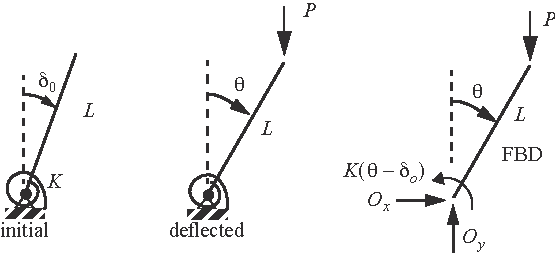
\includegraphics{Figure_10-10.pdf}
}{\caption{Model A with an initial angle.\label{fig10.10}}}
\vspace*{-2\baselineskip}
\begin{align}\label{eq10.39}
P L \sin \theta-K\left(\theta-\delta_{0}\right)=0.
\end{align}
\noindent
Equilibrium equation (\ref{eq10.39}) is plotted in figure~\ref{fig10.11}. The response of model A with the initial angle is similar to the response of model A subject to the eccentric load in figure~\ref{fig10.9}.

\subsubsection{Discussion.} Eccentricity in load and the initial slope of the bar are examples of \textbf{imperfections}. The structural systems are imperfect. Small imperfections of model A do not change the fact that there are large displacements when $P=P_{\mathrm{cr}}$ of the perfect system. Model A is classified as \textbf{stable symmetric bifurcation}. The secondary equilibrium path $p2$ of the perfect system in figure~\ref{fig10.2} is symmetric about $\theta = 0$ and it is stable.

Real structures exhibiting stable symmetric bifurcation are,
\begin{enumerate}
  \item[a.] long straight columns subject to axial compression, and
  \item[b.] flat plates subject to in-plane edge loading.
\end{enumerate}

{\def\thefigure{10.11}
\processfigure{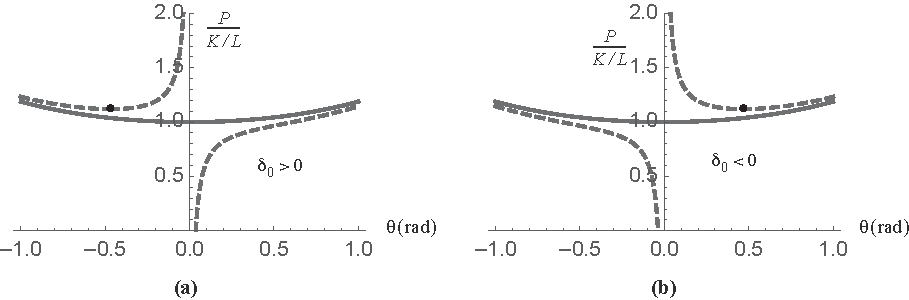
\includegraphics{Figure_10-11.pdf}
}{\caption{Load-deflection plots for model A with the initial angle are shown by the dashed lines for
(a) $\boldsymbol{\delta}_{\textbf{0}}\ \boldmath{>}\ \textbf{0}$ and (b) $\boldsymbol{\delta}_{\textbf{0}}\ \boldmath{<}\ \textbf{0}$.\label{fig10.11}}}}

\vspace*{-0.6pc}

\section{Model B: unstable symmetric bifurcation}\label{sec10.2}

This model consists of a coplanar arrangement of two rigid bars of length \textit{L} and a linear elastic spring of stiffness \textit{K}. The bars are horizontal in the initial position and connect to a center hinge, with the opposite ends of each bar supported on roller support. The vertical spring connects to the center hinge and is not stretched when the bars are in the horizontal position. A horizontal load \textit{P} acts at each roller support to subject the model to compression.

{\def\thefigure{10.12}
\processfigure{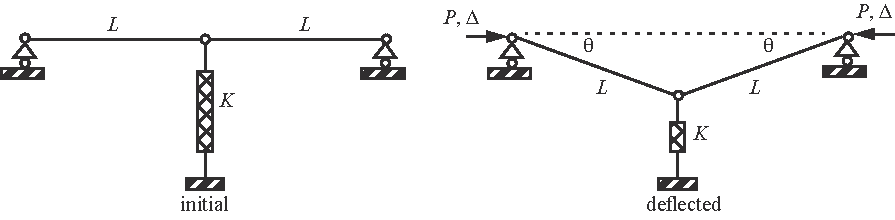
\includegraphics{Figure_10-12.pdf}
}{\caption{Model B.\label{fig10.12}}}}

The deflected configuration of the model is symmetric with respect to the vertical line through the spring, and each bar rotates through an angle $\theta$ with respect to the original horizontal position. The deflection of the spring is $L \sin \theta$, and the load \textit{P} is independent of the corresponding displacement $\Delta(\theta)$. The potential energy is
\begin{align}\label{eq10.40}
V=\frac{1}{2} K(L \sin \theta)^{2}-2 P \underbrace{[L(1-\cos \theta)]}_{\Delta}.
\end{align}
The potential energy is stationary at equilibrium, or $\frac{d V}{d \theta}=0$, which leads to
\begin{align}\label{eq10.41}
(K L^{2} \cos \theta-2 P L) \sin \theta=0.
\end{align}
The solutions of eq.~(\ref{eq10.41}) are
\begin{align}\label{eq10.42}
p 1: \theta=0 \text { for any } P \quad p 2: P=\frac{1}{2} K L \cos \theta.
\end{align}
The equilibrium paths are shown on the load-deflection plot in figure~\ref{fig10.13}. Equilibrium paths intersect at the bifurcation point $(\theta,\; P)=(0,\; \textit{KL}/2)$. By the equilibrium method the critical load is $P_{\mathrm{cr}}=K L / 2$. However, equilibrium states in figure~\ref{fig10.13} are different than those of model A shown in figure~\ref{fig10.2}. Note that there are three equilibrium positions for $P<P_{\mathrm{cr}}$.

{\def\thefigure{10.13}
\processfigure{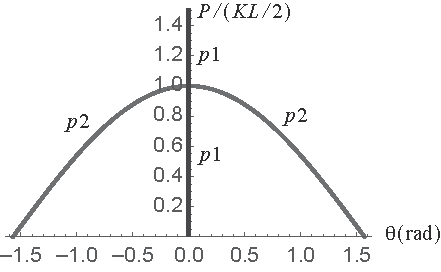
\includegraphics{Figure_10-13.pdf}
}{\caption{Model B equilibrium states.\label{fig10.13}}}}

The stability of the equilibrium states is assessed from the second derivative of the potential energy (\ref{eq10.40}). The second derivative is
\begin{align}\label{eq10.43}
\frac{d^{2} V}{d \theta^{2}}=V_{2}(\theta)=K L^{2}(\cos ^{2} \theta-\sin ^{2} \theta)-2 P L \cos \theta=K L^{2} \cos 2 \theta-2 P L \cos \theta.
\end{align}
On equilibrium path \textit{p1}
\begin{align}\label{eq10.44}
V_{2}(0)=K L^{2}-2 P L.
\end{align}
Therefore, on equilibrium path \textit{p1}
\begin{align}\label{eq10.45}
V_{2}(0)|_{p 1}>0 \text {, stable, } P<\frac{K L}{2} \quad V_{2}(0)|_{p 1}=0, \text { critical, } P=\frac{K L}{2} \quad V_{2}(0)|_{p 1}<0 \text {, unstable, } P>\frac{K L}{2}.
\end{align}
On equilibrium path \textit{p2 }$P=(K L / 2) \cos \theta_{0}$\textit{. }The second derivative is
\begin{align}\label{eq10.46}
V_{2}\left(\theta_{0}\right)=K L^{2}(\cos ^{2} \theta-\sin ^{2} \theta)-2(K L / 2) \cos ^{2} \theta=-K L^{2} \sin ^{2} \theta_{0}.
\end{align}
Therefore, on equilibrium path \textit{p2}
\begin{align}\label{eq10.47}
&V_{2}\left(\theta_{0}\right)|_{p 2}>0, \text { stable, for no } 0<|\theta_{0}| \leq\frac{\pi}{2} \quad V_{2}\left(\theta_{0}\right)|_{p 2}=0, \text { critical, } \theta_{0}=0 \nonumber\\ &V_{2}\left(\theta_{0}\right)|_{p 2}<0, \text { unstable, } 0<|\theta_{0}| \leq \frac{\pi}{2}.
\end{align}
At the bifurcation point $\left(\theta_{0}, P\right)=(0, K L / 2)$ on path \textit{p2} the derivatives of the potential energy are
\begin{align}\label{eq10.48}
V_{2}(0)=0 \quad V_{3}(0)=0 \quad V_{4}(0)=-3 K L^{2}.
\end{align}
The potential energy is a relative maximum at the bifurcation point, so the bifurcation point is unstable. Model B exhibits \textbf{unstable symmetric bifurcation}.


\subsection{Initial angle imperfection}\label{sec10.2.1}

Consider a small deviation of the bars from the horizontal position represented by angle $\delta_{0}$ as shown in figure~\ref{fig10.14}. The spring is not stretched in the initial position.

{\def\floatbelowskip{-3pt}%
\def\thefigure{10.14}
\processfigure{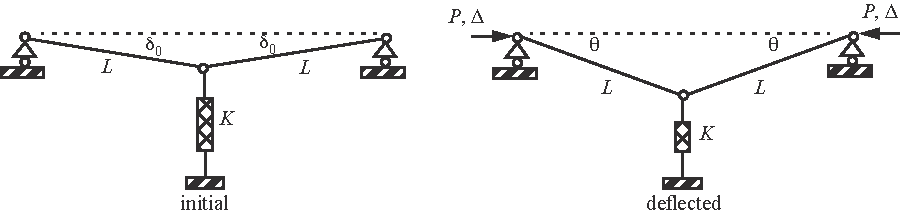
\includegraphics{Figure_10-14.pdf}
}{\caption{Imperfect model B.\label{fig10.14}}}}

\noindent The potential energy of the system is
\begin{align}\label{eq10.49}
V=\frac{1}{2} K\left(L \sin \theta-L \sin \delta_{0}\right)^{2}-2 P L\left(\cos \delta_{0}-\cos \theta\right).
\end{align}
The potential energy is stationary at equilibrium, or $\frac{d V}{d \theta}=0$. Hence, the equilibrium equation is
\begin{align}\label{eq10.50}
K L^{2}\left(\sin \theta-\sin \delta_{0}\right) \cos \theta-2 P L \sin \theta=0.
\end{align}
Equation (\ref{eq10.50}) is written in the equivalent form as
\begin{align}\label{eq10.51}
\left(\sin \theta-\sin \delta_{0}\right) \cos \theta-\left(P / P_{\mathrm{cr}}\right) \sin \theta=0,
\end{align}
where the critical load of the perfect system is $P_{\mathrm{cr}}=K L / 2$. One solution to eq.~(\ref{eq10.51}) is the unloaded state at $(\theta, P)=\left(\delta_{0}, 0\right)$. Other solutions are plotted as dashed lines in the load-deflection plane of figure~\ref{fig10.15}. Equilibrium states along the path beginning at the unloaded state are stable until a relative maximum on the path is encountered at $\left(\theta_{\mathrm{m}}, P_{\mathrm{m}}\right)$, which is indicated by the filled circles in figure~\ref{fig10.15}. There are no stable adjacent equilibrium states if the load \textit{P} increases from $P_{\mathrm{m}}$ or if $\theta$ is increases from $\theta_{\mathrm{m}}$. Any small increase in load or rotation from the relative maximum results in a dynamic motion of the system that may lead to catastrophic collapse.

{\def\thefigure{10.15}
\processfigure{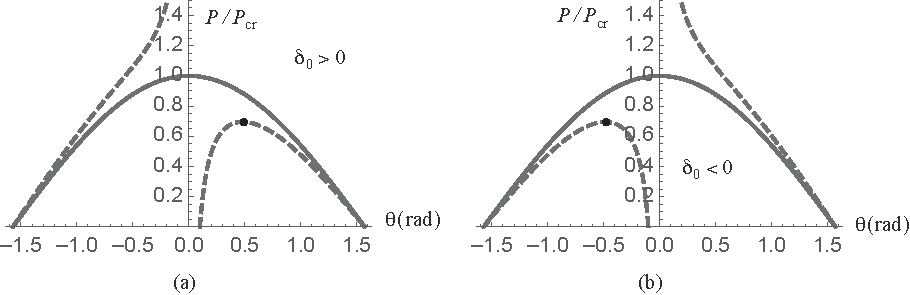
\includegraphics{Figure_10-15.pdf}
}{\caption{Equilibrium paths of the imperfect model B are shown in the load-deflection plane by
dashed lines for (a) $\boldsymbol{\delta}_\textbf{0} \boldsymbol{>} \textbf{0}$ and (b) $\boldsymbol{\delta}_\textbf{0} \boldsymbol{<} \textbf{0}$.\label{fig10.15}}}}


The relative maximum on the equilibrium path emanating from the unloaded state is determined from
\begin{align}\label{eq10.52}
\left(\sin \theta_{\mathrm{m}}-\sin \delta_{0}\right) \cos \theta_{\mathrm{m}}-\left(P_{\mathrm{m}} / P_{\mathrm{cr}}\right) \sin \theta_{\mathrm{m}}=0, \text{where}\ \sin \theta_{\mathrm{m}}=\sqrt[3]{\sin \delta_{0}}.
\end{align}
For selected values of angle $\delta_{0}$ the values of $P_{\mathrm{m}} / P_{\mathrm{cr}}$ are plotted from eq.~(\ref{eq10.52}) in figure~\ref{fig10.16}. There is a rapid decrease in the maximum load for small increases in the imperfection angle. For example, at $\delta_{0}=0.1\,\mathrm{rad}$ ($5.7^{\circ}$) $P_{\mathrm{m}} / P_{\mathrm{cr}}=0.70$, which is a 30\% reduction of the buckling load with respect to the perfect system. For $\delta_{0}=0.1\,\mathrm{rad}$, the value of $\theta_{\mathrm{m}}=0.482\,\mathrm{rad}$, or $27.6^{\circ}$, which is a large rotation at the maximum load.

{\def\thefigure{10.16}
\processfigure{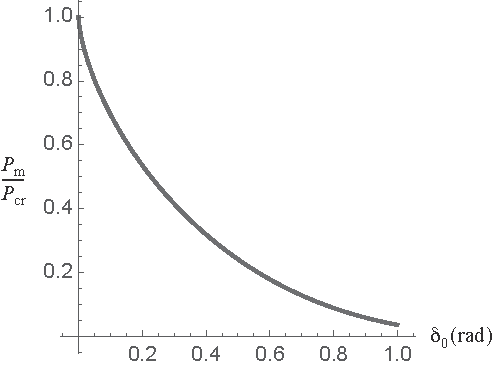
\includegraphics{Figure_10-16.pdf}
}{\caption{The maximum load as a function of the imperfection angle for model B.\label{fig10.16}}}}
\vspace*{-1\baselineskip}

\subsubsection{Discussion.} All real structures are imperfect. For columns and plates these imperfections if small did not significantly reduce the actual buckling load from the critical load $P_{\mathrm{cr}}$ obtained in the analysis of the perfect structure. However, the buckling loads for axially compressed cylindrical shells in experiments are significantly less than the critical load determined from the perfect analysis (small displacements and slopes). Refer to Brush and Almroth (1975). Even for small imperfections in axially compressed shells the maximum load $P_{\mathrm{m}}$ is much lower than $P_{\mathrm{cr}}$. The axially compressed cylindrical shell is sensitive to imperfections.

Is is concluded then, that the value of $P_{\mathrm{cr}}$ may not be meaningful in practice. It depends on the nonlinear behavior of the equilibrium paths.
\begin{itemize}
  \item Model B is imperfection sensitive.
  \item Model A is imperfection insensitive.
\end{itemize}

\clearpage

The question of whether a structure is imperfection sensitive is answered completely by the stability~or~in\-stability~of the bifurcation point or by the initial, nonlinear post-buckling path.

\section{Model C: asymmetric bifurcation}\label{sec10.3}

Model C is a coplanar arrangement of two rigid bars of length \textit{L} and a linear elastic spring with stiffness \textit{K}. In the initial configuration the bars are horizontal and the spring is at a $45^{\circ}$ angle with respect to the bars. The bars and the spring are connected to a smooth central pin. The opposite end of the left bar is pinned to a fixed point, and the opposite end of the spring is connected to a fixed pin at distance \textit{L} below the fixed end of the left bar. The opposite end of the right bar is pinned to a roller support free to move horizontally. A compressive force \textit{P} acts at the roller support and under its action the bars can rotated through an angle $\theta$ with respect to the original horizontal position.

{\def\thefigure{10.17}
\processfigure{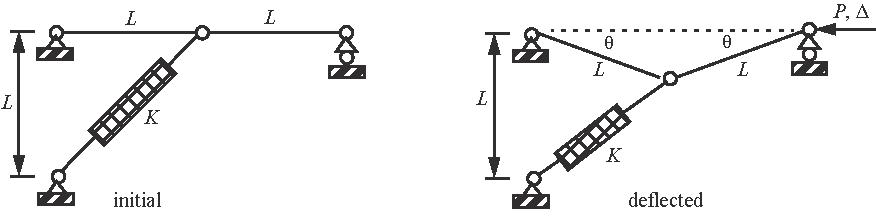
\includegraphics{Figure_10-17.pdf}
}{\caption{Model C.\label{fig10.17}}}}



\noindent The potential energy is $V=K \Delta_{s}^{2} / 2-P \Delta$, where $\Delta_{s}$ denotes the change in the length of the spring and $\Delta$ denotes the shortening of the distance between supports. These changes in length are related to angle $\theta$ by
\begin{align}\label{eq10.53}
\Delta_{s}=\sqrt{(L \cos \theta)^{2}+(L-L \sin \theta)^{2}}-\sqrt{2} L=\sqrt{2} L(\sqrt{1-\sin \theta}-1) \quad \Delta=2 L-2 L \cos \theta.
\end{align}
The total potential energy $V(\theta)$ is given by
\begin{align}\label{eq10.54}
V(\theta)=K L^{2}(\sqrt{1-\sin \theta}-1)^{2}-2 P L(1-\cos \theta).
\end{align}
The potential energy is stationary at equilibrium which leads to
\begin{align}\label{eq10.55}
K L^{2} \cos \theta[(1-\sin \theta)^{-1 / 2}-1]-2 P L \sin \theta=0.
\end{align}
The solutions of eq.~(\ref{eq10.55}) are
\begin{align}\label{eq10.56}
p 1: \theta=0 \text { for any } P \quad p 2: P=\frac{K L}{2} \cot \theta[(1-\sin \theta)^{-1 / 2}-1].
\end{align}
On path \textit{p2} as $\theta \rightarrow 0$, we get the indeterminate form $\frac{K L}{2} \frac{1}{0}\left(\frac{1}{1}-1\right)=\frac{K L}{2} \frac{1}{0} \times 0$. The limit of this indeterminate form is found from l'H\^{o}pital's rule to be
\begin{align}\label{eq10.57}
P=P_{\mathrm{cr}}=K L / 4\quad \text {at } \theta=0.
\end{align}
The equilibrium paths are plotted on the load-deflection plane in figure~\ref{fig10.18}. Equilibrium path \textit{p2} is asymmetric about $\theta = 0$. Stability analysis leads to path \textit{p2} being stable for $\theta > 0$ and unstable for $\theta < 0$. Path \textit{p1} is stable for $0 \leq P<P_{\mathrm{cr}}$ and unstable for $P>P_{\mathrm{cr}}$. At the bifurcation point $(\theta, P)=\left(0, P_{\mathrm{cr}}\right)$ higher derivatives of the potential energy are $V_{2}=0$ and $V_{3}=\left(3 K L^{2}\right) / 4$. That is, the potential energy is neither a minimum nor maximum, but has a horizontal inflection point at $(\theta, P)=\left(0, P_{\mathrm{cr}}\right)$.

{\def\thefigure{10.18}
\processfigure{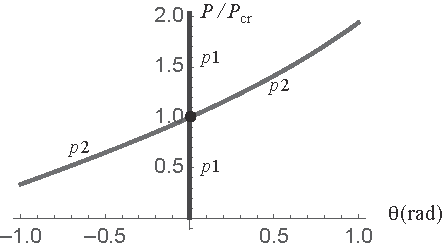
\includegraphics{Figure_10-18.pdf}
}{\caption{Model C equilibrium states.\label{fig10.18}}}}

\begin{wrapfigure}[10]{r}{154pt}
%\vspace{-19pt}
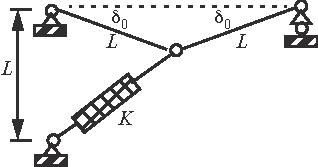
\includegraphics{Figure_10-19.pdf}
\caption{Imperfect model C.\label{fig10.19}}
\end{wrapfigure}
{\def\thefigure{10.20}
\processfigure[b]{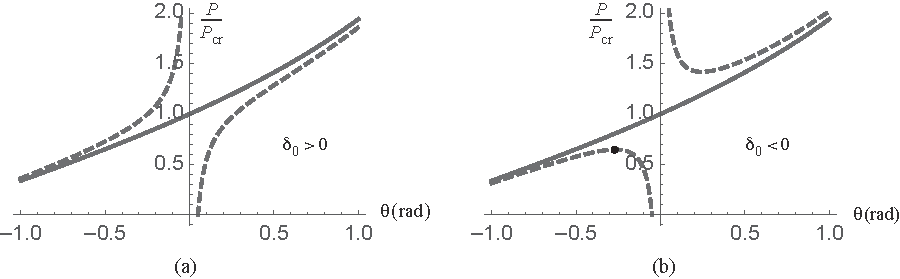
\includegraphics{Figure_10-20.pdf}
}{\caption{Equilibrium paths of the imperfect model C shown as dashed lines for (a) $\boldsymbol{\delta}_\textbf{0} \boldsymbol{>} \textbf{0}$ and (b) ${\boldsymbol{\delta}_\textbf{0} \boldsymbol{<} \textbf{0}}$.\label{fig10.20}}\vspace*{14pt}}}

Consider a geometric imperfection of model C in which the bars are at an angle $\delta_{0}$ with respect to the horizontal before the load is applied as is shown in figure~\ref{fig10.19}. In the unloaded configuration the spring is not stretched nor contracted. The change in spring length is
\begin{align}\label{eq10.58}
\Delta_{s}=\sqrt{2} L\left(\sqrt{1-\sin \theta}-\sqrt{1-\sin \delta_{0}}\hspace*{3pt}\right).
\end{align}
The potential energy is
\begin{align}\label{eq10.59}
V=K L^{2}\left(\sqrt{1-\sin \theta}-\sqrt{1-\sin \delta_{0}}\hspace*{3pt}\right)^{2}-2 P L\left(\cos \delta_{0}-\cos \theta\right).
\end{align}
The potential energy is stationary at equilibrium, which leads to
\begin{align}\label{eq10.60}
K L^{2} \cos \theta\left(\frac{\sqrt{1-\sin \theta}-\sqrt{1-\sin \delta_{0}}}{\sqrt{1-\sin \theta}}\right)-2 P L \sin \theta=0.
\end{align}
Solve eq.~(\ref{eq10.60}) for \textit{P} and divide by $P_{\mathrm{cr}}=K L / 4$ to get\enlargethispage{1\baselineskip}
\begin{align}\label{eq10.61}
\frac{P}{P_{\mathrm{cr}}}=2 \cot \theta\left(\frac{\sqrt{1-\sin \theta}-\sqrt{1-\sin \delta_{0}}}{\sqrt{1-\sin \theta}}\right).
\end{align}
Note that a solution of eq.~(\ref{eq10.61}) is $(\theta, P)=\left(\delta_{0}, 0\right)$. The equilibrium paths determined from eq.~(\ref{eq10.61}) are shown as dashed lines in the load-deflection plane of figure~\ref{fig10.20}. The equilibrium path beginning at the\vadjust{\pagebreak} unloaded state for $\delta_{0}>0$ in figure~\ref{fig10.20}(a) is stable and the deflection increases rapidly as the load approaches the critical load of the perfect system. The equilibrium path beginning at the unloaded state for $\delta_{0}<0$ in figure~\ref{fig10.20}(b) is stable until the maximum load $P_{\mathrm{m}}$ is encountered, which is indicated by the filled circle. There are no stable adjacent equilibrium states if \textit{P} is increased from $P_{\mathrm{m}}$ or if $\theta$ decreases from the maximum load point. Hence, model C is imperfection sensitive for $\delta_{0}<0$.


\begin{wrapfigure}[9]{r}{141pt}
\vspace{-19pt}
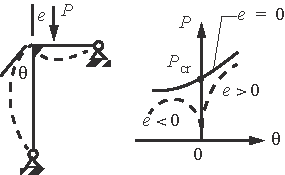
\includegraphics{Figure_10-21.pdf}
\caption{A frame of two members supported by smooth pins.\label{fig10.21}}
\end{wrapfigure}

A real structure exhibiting asymmetric bifurcation is a pin-supported, two-member frame. The joint connecting the members is assumed rigid. Thus, each bar rotates through the same angle at the joint as shown in figure~\ref{fig10.21}. For $e>0$ the horizontal member is in tension, which is a stabilizing effect. For $e<0$ the horizontal member is in compression, which is a destabilizing effect.

\section{Discussion of models A, B, and C}\label{sec10.4}

\def\rightmark{Model D: snap-through instability}

We have considered three one-degree-of-freedom models (one coordinate is sufficient to describe the equilibrium configuration). The equilibrium paths were plotted on the $(\theta, P)$ plane. For the perfect system $\theta = 0$ for any \textit{P} is an equilibrium state (trivial equilibrium). Two equilibrium paths of the perfect system cross at the \textbf{bifurcation point} $(\theta, P)=\left(0, P_{\mathrm{cr}}\right)$. There are three basic bifurcation points: stable symmetric, unstable symmetric, and asymmetric. The unstable symmetric and asymmetric cases are \textbf{imperfection sensitive}. A maximum load $P_{\mathrm{m}}$ below $P_{\mathrm{cr}}$ is possible when the system has imperfections. This theory was originally developed in the PhD dissertation by Koiter (1945 in Dutch, English translation 1970).

\section{Model D: snap-through instability}\label{sec10.5}

Model D is a coplanar arrangement of two rigid bars and a linear elastic spring in the shape of an arch as shown in figure~\ref{fig10.22}. Each bar has the same length \textit{L}, and the bars connect to a central pin. The bars are at angle $\alpha$ with respect to a horizontal line passing through the supported ends of the bars. The left end of the left bar is pin-connected to a fixed support. The right end of the right bar is pin-connected to a roller support restrained to move horizontally by a linear elastic spring with stiffness \textit{K}. The model is subject to a downward, deadweight load \textit{P} acting at the central pin.

{\def\thefigure{10.22}
\processfigure{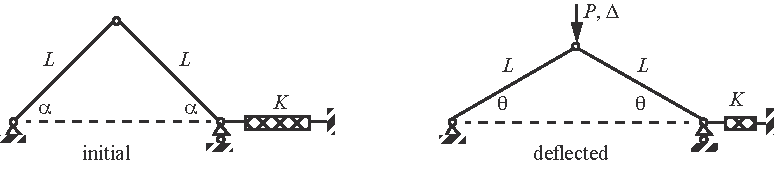
\includegraphics{Figure_10-22.pdf}
}{\caption{Model D.\label{fig10.22}}}}

The total potential energy is $V=K\left(\Delta_{s}\right)^{2 / 2-P \Delta}$, where $\Delta_{s}$ is the change in length of the spring and $\Delta$ is the downward displacement corresponding to the load \textit{P}. The change in length of the spring and the downward displacement~are\vspace*{-6pt}
\begin{align}\label{eq10.62}
\Delta_{s}=2 L(\cos \theta-\cos \alpha) \quad \Delta=L(\sin \alpha-\sin \theta).
\end{align}
Hence, the total potential energy is
\begin{align}\label{eq10.63}
V(\theta)=2 K L^{2}(\cos \theta-\cos \alpha)^{2}-P L(\sin \alpha-\sin \theta).
\end{align}
The total potential energy is stationary at equilibrium, which yields the equilibrium equation
\begin{align}\label{eq10.64}
4 K L^{2}(\cos \theta-\cos \alpha)(-\sin \theta)+P L \cos \theta=0.
\end{align}
Solve eq.~(\ref{eq10.64}) for load \textit{P} to get
\begin{align}\label{eq10.65}
P=4 K L(\cos \theta-\cos \alpha) \tan \theta.
\end{align}
Note that the range of $\theta$ in eq.~(\ref{eq10.65}) is $-\pi / 2<\theta<\pi / 2$ for finite values of the load \textit{P.} On a plot of the load \textit{P} as a function of $\theta$, horizontal slopes occur at $\frac{d P}{d \theta}=0$. The derivative of eq.~(\ref{eq10.65}) with respect to $\theta$ is
\begin{align}\label{eq10.66}
\frac{d P}{d \theta}=4 K L\left[-\sin \theta \tan \theta+\frac{(\cos \theta-\cos \alpha)}{\cos ^{2} \theta}\right]=4 K L \frac{(\cos ^{3} \theta-\cos \alpha)}{\cos ^{2} \theta}.
\end{align}
Therefore horizontal slopes occur at
\begin{align}\label{eq10.67}
\theta_{\mathrm{m}}=\pm \operatorname{acos}[\sqrt[3]{\cos \alpha}],
\end{align}
Substitute $\cos \theta=\cos ^{1 / 3} \alpha$ into eq.~(\ref{eq10.65}) and use trigonometric identities to find the load at the horizontal slope to be
\begin{align}\label{eq10.68}
P_{\mathrm{m}}=4 K L(1-\cos ^{2 / 3} \alpha)^{3 / 2}.
\end{align}
For $\alpha=45^{\circ}$, $\theta_{\mathrm{m}}=\pm 27.01^{\circ}$. At $\theta_{\mathrm{m}}=-27.01^{\circ}$ the load $P_{\mathrm{m}}=-0.375\,KL$ with the corresponding displacement $\Delta_{\mathrm{m}}=1.16\,{L}$. At $\theta_{\mathrm{m}}=27.01^{\circ}$ the load $P_{\mathrm{m}}=0.375\,{KL}$ with the corresponding displacement $\Delta_{\mathrm{m}}=0.253\,{L}$. The load-displacement response is plotted in figure~\ref{fig10.23} by selecting $\theta$ and computing \textit{P} from eq.~(\ref{eq10.65}) and $\Delta$ from eq.~(\ref{eq10.62}). There is one continuous path with no bifurcation. The loads at the horizontal slopes are indicated by filled circles in figure~\ref{fig10.23}.

{\def\thefigure{10.23}
\processfigure{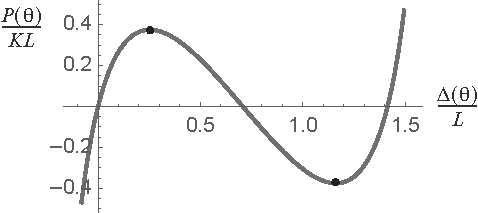
\includegraphics{Figure_10-23.pdf}
}{\caption{Equilibrium path on the load\break displacement plane for model D. $|\theta|\leq \textbf{52}^\circ$
and $\alpha = \textbf{45}^\circ$.\label{fig10.23}}}}

The stability of the equilibrium states are determined from the second derivative of the potential energy. The second derivative is
\begin{align}\label{eq10.69}
\frac{d^{2} V}{d \theta^{2}}=4 K L^{2}[\sin ^{2} \theta-\cos \theta(-\cos \alpha+\cos \theta)]-P L \sin \theta.
\end{align}
\vspace*{5pt}
\clearpage

\noindent Substitute the expression for \textit{P} from eq.~(\ref{eq10.65}) into eq.~(\ref{eq10.69}) to evaluate the second derivative on the equilibrium path to find
\begin{align}\label{eq10.70}
V_{2}(\theta)=\frac{d^{2} V}{d \theta^{2}}=4 K L^{2} \frac{\left(\cos ^{3} \theta-\cos \alpha\right)}{\cos \theta}.
\end{align}
For $|\theta|<\pi / 2$, $\cos \theta>0$. Select a value of $\theta$ in the range $|\theta|<\pi / 2$. Then, the value of $\Delta$ is computed from eq.~(\ref{eq10.62}) and the value of the second derivative of the potential energy is computed from eq.~(\ref{eq10.70}). The plot of the second derivative divided by $K L^{2}$ with respect to $\Delta / L$ is shown in figure~\ref{fig10.24}.

{\def\thefigure{10.24}
\processfigure{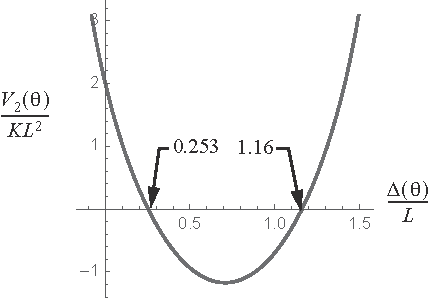
\includegraphics{Figure_10-24.pdf}}{\caption{Parametric plot of the second derivative of the potential energy with respect to the displacement along the equilibrium path for model D. $\boldmath{|\theta|\leq \textbf{52}^\circ}$
and $\boldsymbol{\alpha} \boldsymbol{=} {\textbf{45}}^{\boldsymbol{\circ}}$.\label{fig10.24}}}}
{\def\thefigure{10.25}
\processfigure[b]{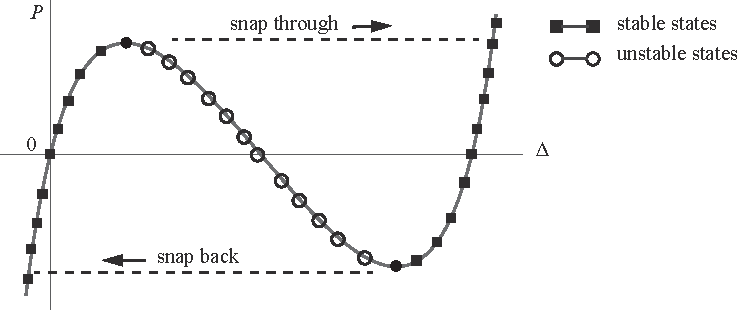
\includegraphics{Figure_10-25.pdf}
}{\caption{Stability of the equilibrium path for model~D.
$\boldmath{\alpha}\ \boldmath{=}\  \textbf{45}^{\boldsymbol{\circ}}$.\label{fig10.25}}}}

\noindent For $\alpha=45^{\circ}$ the range of $\Delta$ is $-0.2929 L<\Delta<1.707 L$ when $\theta$ is in the interval $\pi / 2>\theta>-\pi / 2$. From figure~\ref{fig10.24} the stability of the equilibrium path is determined as
\begin{gather}\label{eq10.71}
V_{2}>0, \text { stable, }-0.293<\Delta / L<0.253\, \&\, 1.16<\Delta / L<1.1707,
\\\label{eq10.72}
V_{2}=0 \text {, critical } \Delta / L=0.253\, \&\, \Delta / L=1.16, \text{and}
\\
\label{eq10.73}
V_{2}<0, \text { unstable, } 0.253<\Delta / L<1.16.
\end{gather}
The stability of the equilibrium path is depicted in figure~\ref{fig10.25}. As the load \textit{P} is increased from $\Delta=0$ a maximum load $P_{\mathrm{m}}$ is encountered. If the load is increased further the system snaps-through. The maximum point is called\vadjust{\pagebreak} a \textbf{limit point}. This is a different kind of instability from the perfect systems of models A, B, and C. In models A, B, and C $\theta = 0$ was an equilibrium state of the perfect system. Model D is said to have pre-buckling ``deformations.'' That is $\theta \neq 0$ before buckling. Snap-through is a dynamic event, and the system can settle to an inverted, stable equilibrium state. If the load is decreased from the inverted state to the lower limit point the system can snap back to a shape resembling the original configuration.

\def\rightmark{Model E: a two-degree-of freedom system}

\section{Model E: a two-degree-of freedom system}\label{sec10.6}

Models A to D are single-degree-of-freedom systems. Only one coordinate $\theta$ determines the position of the system. Consider a two-degree-of-freedom system consisting of rigid bar restrained by two rotational springs with stiffnesses $\textit{K}_1$ and $\textit{K}_2$, and subject to a vertical, deadweight load \textit{P} as shown in figure~\ref{fig10.26}. This model is known as Augusti's column. See Bazant and Cedolin (1991). The position of the bar is referenced to a right-handed Cartesian coordinate system \textit{x-y-z}, with corresponding unit vectors $\hat{i}, \hat{j}, \hat{k}$. The initial position of the bar is vertical coinciding with the $z$-axis shown in figure~\ref{fig10.26}(a), and in the deflected position it is located by two angles $\theta_1$ and $\theta_2$ shown in figure~\ref{fig10.26}(b) The projection of the bar into the \textit{x-z} plane is at angle $\theta_1$ with respect to the $z$-axis. The projection of the bar in the \textit{y-z} plane is at angle $\theta_2$ with respect to the $z$-axis.

{\def\thefigure{10.26}
\processfigure{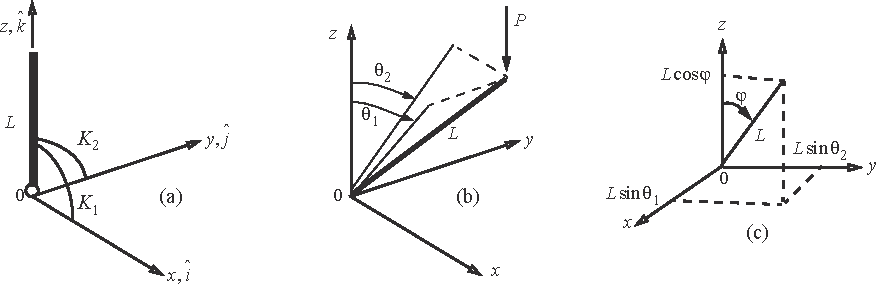
\includegraphics{Figure_10-26.pdf}
}{\caption{Model E. (a) Initial unloaded configuration. (b) Deflected configuration
under a downward applied load. (c) Coordinates at end of the bar.\label{fig10.26}}}}

The angle between the bar and the $z$-axis is denoted by $\varphi$. The Cartesian coordinates at the end of the bar in its deflected position in shown in figure~\ref{fig10.26} (c) are $\left(L \sin \theta_{1}, L \sin \theta_{2}, L \cos \varphi\right)$. By the Pythagorean theorem the square of the length of the bar in the deflected position is given by
\begin{align}\label{eq10.74}
L^{2}=\left(L \sin \theta_{1}\right)^{2}+\left(L \sin \theta_{2}\right)^{2}+(L \cos \varphi)^{2}.
\end{align}
From eq.~(\ref{eq10.74}) we find that the cosine of the angle $\varphi$ is
\begin{align}\label{eq10.75}
\cos \varphi=\sqrt{1-\sin ^{2} \theta_{1}-\sin ^{2} \theta_{2}}.
\end{align}
The displacement corresponding to load \textit{P} is $\Delta=L(1-\cos \varphi)$. The total potential energy is
\begin{align}\label{eq10.76}
V\left(\theta_{1}, \theta_{2}\right)=K_{1} \theta_{1}^{2} / 2+K_{2} \theta_{1}^{2} / 2-P L\left(1-\sqrt{1-\sin ^{2} \theta_{1}-\sin ^{2} \theta_{2}}\hspace*{4pt}\right).
\end{align}
The series expansion of $1-\cos \varphi$ is
\begin{align}\label{eq10.77}
1-\sqrt{1-\sin ^{2} \theta_{1}-\sin ^{2} \theta_{2}}=\frac{1}{2}\left(\theta_{1}^{2}+\theta_{2}^{2}+\frac{1}{2} \theta_{1}^{2} \theta_{2}^{2}-\frac{1}{12} \theta_{1}^{4}-\frac{1}{12} \theta_{2}^{4}+O(\theta^{6})\right).
\end{align}
Neglect terms of order six and higher in the series expansion to get the total potential energy as
\begin{align}\label{eq10.78}
V\left(\theta_{1}, \theta_{2}\right)=K_{1} \theta_{1}^{2} / 2+K_{2} \theta_{1}^{2} / 2-P L\left(\theta_{1}^{2}+\theta_{2}^{2}+\frac{1}{2} \theta_{1}^{2} \theta_{2}^{2}-\frac{1}{12} \theta_{1}^{4}-\frac{1}{12} \theta_{2}^{4}\right) / 2.
\end{align}

\vspace*{-1pc}

Let $\theta_{1}=\theta_{10}$ and $\theta_{2}=\theta_{20}$ denote the angles in an equilibrium state, and let small changes in the angles with respect to the equilibrium state be denoted by
\begin{align}\label{eq10.79}
h_{1}=\theta_{1}-\theta_{10} \quad \text { and } \quad h_{2}=\theta_{2}-\theta_{20}.
\end{align}
The Taylor series of the potential energy about the equilibrium state is
\begin{align}\label{eq10.80}
V\left(\theta_{1}, \theta_{2}\right)=V\left(\theta_{10}, \theta_{20}\right)+\delta V+\delta^{2} V+\delta^{3} V+\delta^{4} V+\ldots,
\end{align}
where $\delta V$ is called the first variation with terms linear in $h_1$ and $h_2$, and $\delta^{2} V$ is called the second variation with terms quadratic in $h_1$ and $h_2$, etc. The change in potential energy about the equilibrium state is $\Delta V=V\left(\theta_{1}, \theta_{2}\right)-V\left(\theta_{10}, \theta_{20}\right)$. Thus,
\begin{align}\label{eq10.81}
\Delta V=\delta V+\delta^{2} V+\delta^{3} V+\delta^{4} V+\ldots.
\end{align}
Partial derivatives of the potential energy evaluated at the equilibrium state are represented by the notation
\begin{align}\label{eq10.82}
V_{0}^{(m, n)}=\left.\frac{\partial^{(m\,{+}\,n)} V}{\partial \theta_{1}^{m} \partial \theta_{2}^{n}}\right|_{\theta_{10}, \theta_{20}} \quad m, n=0,1,2, \ldots.
\end{align}
For example,
\begin{align}\label{eq10.83}
V_{0}^{(1,0)}=\left.\frac{\partial V}{\partial \theta_{1}}\right|_{\theta_{10}, \theta_{20}} \quad V_{0}^{(1,1)}=\left.\frac{\partial^{2} V}{\partial \theta_{1} \partial \theta_{2}}\right|_{\theta_{10}, \theta_{20}} \quad V_{0}^{(2,2)}=\left.\frac{\partial^{4} V}{\partial \theta_{1}^{2} \partial \theta_{2}^{2}}\right|_{\theta_{10}, \theta_{20}}.
\end{align}
The terms in the Taylor series expansion (\ref{eq10.81}) are
\begin{align}\label{eq10.84}
\begin{gathered}
\delta V=V_{0}^{(1,0)} h_{1}+V_{0}^{(0,1)} h_{2} \\
\delta^{2} V=\frac{1}{2}\left(V_{0}^{(2,0)} h_{1}^{2}+2 V_{0}^{(1,1)} h_{1} h_{2}+V_{0}^{(0,2)} h_{2}^{2}\right) \\
\delta^{3} V=\frac{1}{6}\left(V_{0}^{(3,0)} h_{1}^{3}+3 V_{0}^{(2,1)} h_{1}^{2} h_{2}+3 V_0^{(1,2)} h_{1} h_{2}^{2}+V_{0}^{(0,3)} h_{2}^{3}\right) \\
\delta^{4} V=\frac{1}{24}\left(V_{0}^{(4,0)} h_{1}^{4}+4 V_{0}^{(3,1)} h_{1}^{3} h_{2}+6 V_{0}^{(2,2)} h_{1}^{2} h_{2}^{2}+4 V_{0}^{(1,3)} h_{1} h_{2}^{3}+V_{0}^{(0,4)} h_{2}^{4}\right)
\end{gathered}.
\end{align}

\vspace*{-1pc}

A necessary condition for the potential energy to be a relative minimum or maximum at the equilibrium state is $\delta V=0$ for every $h_1$ and $h_2$, but both not equal to zero. Thus, ``coefficients'' $V_{0}^{(1,0)}=0$ and $V_{0}^{(0,1)}=0$. The potential energy is stationary at equilibrium. Take the partial derivatives of the potential energy (\ref{eq10.78}) to get the equilibrium equations
\begin{align}\label{eq10.85}
V_{0}^{(1,0)}=K_{1} \theta_{10}-L P(\theta_{10}-\theta_{10}^{3} / 6+\theta_{10} \theta_{20}^{2} / 2)=0,\ \text{and}
\\
\label{eq10.86}
V_{0}^{(0,1)}=K_{2} \theta_{20}-L P(\theta_{20}-\theta_{20}^{3} / 6+\theta_{10}^{2} \theta_{20} / 2)=0.
\end{align}
A solution to the equilibrium equations (\ref{eq10.85}) and (\ref{eq10.86}) is
\begin{align}\label{eq10.87}
p 1: \theta_{10}=\theta_{20}=0 \text { for any } P.
\end{align}
The next non-zero term in the expansion of $\Delta V$ is the second variation. Evaluating the second order partial derivatives of the potential energy (\ref{eq10.78}) followed by evaluation on equilibrium path \textit{p1} we get
\begin{align}\label{eq10.88}
\delta^{2} V=\frac{1}{2}\left[\left(K_{1}-L P\right) h_{1}^{2}+\left(K_{2}-L P\right) h_{2}^{2}\right].
\end{align}
\begin{wrapfigure}[11]{l}{88pt}
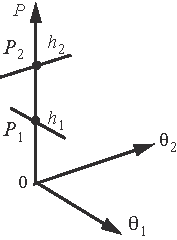
\includegraphics{Figure_10-27.pdf}
\caption{\label{fig10.27}}
\end{wrapfigure}

\vspace*{-1.5pc}

\noindent  Buckling loads are determined when second variation vanishes for every value of $h_1$ and $h_2$, but both not equal to zero. This leads to two buckling loads and associated modes
\begin{align}\label{eq10.89}
P_{1}=K_{1} / L \quad\left(h_{1}, h_{2}\right)=(1,0),\ \text{and}\\
\label{eq10.90}
P_{2}=K_{2} / L \quad\left(h_{1}, h_{2}\right)=(0,1).
\end{align}
The critical loads and modes are shown in the load-deflection plane of figure~\ref{fig10.27}. Take the case of $K_{1}<K_{2}$. Then, the critical load is $P_{\mathrm{cr}}=P_{1}=K_{1} / L$ and the associated mode is $\left(h_{1}, h_{2}\right)=(1,0)$.

The second variation $\delta^{2} V$ is a quadratic form in variables $h_1$ and $h_2$. Examples of quadratic forms and their descriptions are listed in Table \ref{tab10.1}.

\begin{table}[h]
\processtable{Examples of quadratic forms\label{tab10.1}}{%
\tabcolsep=20pt\begin{tabular}{@{}ll@{}}
\toprule
\colhead{$\delta^{2} V$} & \colhead{Description} \\
\midrule
$h^2_1 + h^2_2$ & Positive definite\\
$\left(h_{1}+h_{2}\right)^{2}$ & Positive semidefinite\\
$-h_{1}^{2}-h_{2}^{2}$ & Negative definite\\
$-\left(h_{1}+h_{2}\right)^{2}$ & Negative semidefinite\\
$h_{1} h_{2}$ & Indefinite\\
\botrule
\end{tabular}}{}\vspace*{-13pt}
\end{table}

The second variation (\ref{eq10.88}) is \textbf{positive definite} for $0 \leq P<K_{1} / L$. At the critical load the second variation is
\begin{align}\label{eq10.91}
\delta^{2} V=\frac{1}{2}\left[0 \cdot h_{1}^{2}+\left(K_{2}-K_{1}\right) h_{2}^{2}\right].
\end{align}
The second variation at the critical load is said to be \textbf{positive semidefinite}. It is zero for all non-zero values of $h_1$ and $h_2 = 0$, but is positive for all non-zero values of $h_2$ and $h_1 = 0$. The second variation ceases to be positive definite at the critical state. The stability of equilibrium path $p_{1}$ is determined from eq.~(\ref{eq10.88}) as follows:
\begin{align}\label{eq10.92}
\left.\delta^{2} V\right|_{p 1}>0 \text {, stable, } 0 \leq P<K_{1} /\left.L \quad \delta^{2} V\right|_{p 1}=0 \text {, critical, } P=K_{1} /\left.L \quad \delta^{2} V\right|_{p 1}<0 \text {, unstable, } P>K_{1} / L.
\end{align}
The stability of the bifurcation point $\left(\theta_{1}, \theta_{2}, P\right)=\left(0,0, K_{1} / L\right)$ is not determined from the second variation of the potential energy.

At the critical load $\theta_{2}=0$. This suggests we seek a solution to equilibrium equations (\ref{eq10.85}) and (\ref{eq10.86}) with $\theta_{10} \neq 0$ and $\theta_{20}=0$. Equation (\ref{eq10.86}) is identically satisfied, and eq.~(\ref{eq10.85}) reduces to
\begin{align}\label{eq10.93}
K_{1} \theta_{10}-L P(\theta_{10}-\theta_{10}^{3} / 6)=0.
\end{align}
Solve eq.~(\ref{eq10.93}) for \textit{P} to get
\begin{align}\label{eq10.94}
\frac{P}{P_{\mathrm{cr}}}=\frac{\theta_{10}}{\theta_{10}-\theta_{10}^{3} / 6}.
\end{align}
The equilibrium path described by eq.~(\ref{eq10.94}) is shown in figure~\ref{fig10.28}. The load increases in the initial post-buckling response indicating the bifurcation point is stable.

{\def\thefigure{10.28}
\processfigure[H]{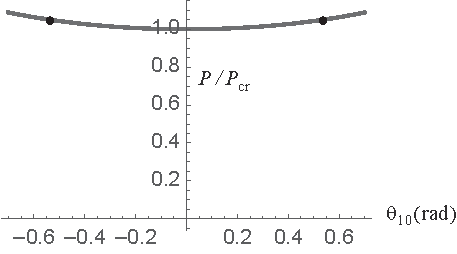
\includegraphics{Figure_10-28.pdf}
}{\caption{Post-buckling equilibrium path for model E with $\boldsymbol{\theta}_{\textbf{20}} \boldsymbol{=} \textbf{0}$ and $K_{\textbf{1}} \boldmath{<} K_{\textbf{2}}$.\label{fig10.28}}}}

Consider the case where $K_{1}=K_{2}=K$. The critical points $\textit{P}_1$ and $\textit{P}_2$ coincide on the path $p_1$ and simultaneous buckling modes $\left(h_{1}, h_{2}\right)=(1,0)$ and $\left(h_{1}, h_{2}\right)=(0,1)$ interact at $\left(\theta_{1}, \theta_{2}, P\right)=(0,0, K / L)$. In this case both $\delta V=0$ and $\delta^{2} V=0$ at the bifurcation point, and we have to consider the next non-zero term in the expansion of the change in potential energy (\ref{eq10.81}). To evaluate the third variation at the bifurcation point, the third partial derivatives of the total potential energy evaluated a the bifurcation point are
\begin{align}\label{eq10.95}
V_{0}^{(3,0)}=V_{0}^{(2,1)}=V_{0}^{(1,2)}=V_{0}^{(0,3)}=0.
\end{align}
Hence, $\delta^{3} V=0$ for all values of $h_1$ and $h_2$. Evaluate the fourth partial derivatives of the total potential energy at the bifurcation point to find
\begin{align}\label{eq10.96}
V_{0}^{(4,0)}=K_{1} \quad V_{0}^{(3,1)}=0 \quad V_{0}^{(2,2)}=-K_{1} \quad V_{0}^{(1,3)}=0 \quad V_{0}^{(0,4)}=K_{1}.
\end{align}
The fourth variation of the potential energy is
\begin{align}\label{eq10.97}
\delta^{4} V=\frac{1}{24}(K_{1} h_{1}^{4}-6 K_{1} h_{1}^{2} h_{2}^{2}+K_{1} h_{2}^{4}).
\end{align}
The fourth variation vanishes at $h_{2}=\pm 0.414 h_{1}$ and $h_{2}=\pm 2.414 h_{1}$. Regions in the $h_1$-$h_2$ plane where the fourth variation is positive and negative are established by plotting the locus where it is zero as shown in figure~\ref{fig10.29}. The minimum values of the fourth variation occur along the directions $h_{2}=\pm \sqrt{3} h_{1}$ and are $\delta^{4} V=-K_{1} h_{1}^{4} / 3$.\vadjust{\pagebreak} Since the fourth variation can be positive, zero, and negative depending on the values of $h_1$ and $h_2$, the fourth variation is \textbf{indefinite}. The bifurcation point is unstable. It is shown in Bazant and Cedolin (1991) that the condition for existence of a non-zero solution to equilibrium equations (\ref{eq10.85}) and (\ref{eq10.86}) is $\theta_{10}=\theta_{20}=\theta$. The two equilibrium equations reduce to the single equation
{\def\thefigure{10.29}
\processfigure[t]{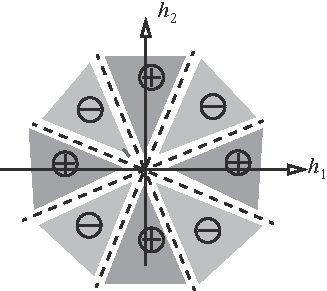
\includegraphics{Figure_10-29.pdf}
}{\caption{Regions in the $h_{\textbf{1}}$-$h_{\textbf{2}}$ plane where the
fourth variation is positive and negative, Along
the dashed lines the fourth variation is zero.\label{fig10.29}}}}
\begin{align}\label{eq10.98}
K \theta-P L(\theta+\theta^{3} / 3)=0.
\end{align}
Solve eq.~(\ref{eq10.98}) for the load \textit{P} to get
\begin{align}\label{eq10.99}
P / P_{\mathrm{cr}}=\frac{\theta}{\theta+\theta^{3} / 3}.
\end{align}
The load decreases from the critical value on the post-buckling path for $|\theta|>0$ as shown in figure~\ref{fig10.30}.

{\def\thefigure{10.30}
\processfigure[H]{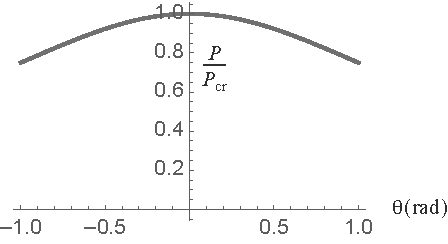
\includegraphics{Figure_10-30.pdf}
}{\caption{Model E post-buckling
equilibrium path for $K_{\textbf{1}} = K_{\textbf{2}}$ and $\theta_{\textbf{1}} =
\theta_{\textbf{2}} = \theta$.\label{fig10.30}}}}

\textbf{For} $\textbf{\textit{K}}_{\textbf{1}} \boldsymbol{<} \textbf{\textit{K}}_{\textbf{2}}$ \textbf{the bifurcation point stable and the system is imperfection insensitive. For} $\textbf{\textit{K}}_{\textbf{1}} \boldsymbol{=} \textbf{\textit{K}}_{\textbf{2}} \boldsymbol{=} \textbf{\textit{K}}$ \textbf{the bifurcation point is unstable and the system is imperfection sensitive.}


\begin{thebibliography}{}\label{sec10.7}
\bibitem{}
Bazant, Z., and L. Cedolin. \textbf{Stability of Structures:} \textbf{Elastic, Inelastic, Fracture, and Damage Theories}. New York: Oxford University Press, 1991, p.265.

\bibitem{}
Brush, D. O., and BO O. Almroth. \textbf{Buckling of Bars, Plates, and Shells}. New York: McGraw-Hill, 1975, p. 185.

\bibitem{}
Huseyin, K. \textbf{Nonlinear theory of elastic stability}. Leyden, The Netherlands: Noordhoff International Publishing, 1975.

\bibitem{}
Koiter, W. T. ``The Stability of Elastic Equilibrium.'' PhD diss., Teehisehe Hoog School, Delft, The Netherlands. 1945. (English translation published as Technical Report AFFDL-TR-70-25, Air Force Flight Dynamics Laboratory, Wright-Patterson Air Force Base, OH, February 1970.)

\bibitem{}
Simitses, G. \textbf{An Introduction to the Elastic Stability of Structures.} Englewood Cliffs, NJ: Prentice Hall, Inc., 1976, Chapter 2.

\bibitem{}
Ziegler, Hans. \textbf{Principles of Structural Stability}. Waltham, Massachusetts: Blaisdell Publishing Company, A Division of Ginn and Company, 1968, Chapter 1.
\end{thebibliography}

\def\rightmark{Practice exercises}

\section{Practice exercises}\label{sec10.8}

\begin{exercise}
\begin{enumerate}[\textbf{2.}]
\item[\textbf{1.}] A rigid, straight bar of length \textit{L} is pinned a point \textit{O}, restrained by a linear elastic spring with stiffness \textit{K}, and subject to a downward load \textit{P}. Neglect the weight of the bar. The bar is vertical in the initial configuration as shown in figure~\ref{fig10.31}(a).The spring remains horizontal as the bar rotates from the vertical through angle $\theta$ as shown in figure~\ref{fig10.31}(b). Refer to the free body diagram in figure~\ref{fig10.31}(c) to find the equation of motion is\vspace*{-0.5pc}
\begin{align}\label{eq10.100}
P L \sin \theta-[K(a \sin \theta)] a \cos \theta=I_{0} \frac{d^{2} \theta}{d t^{2}} \quad \theta=\theta(t),
\end{align}
where ${I_0}$ is the moment of inertia of the rod about the fixed point and $t$ is time. $\theta>0$ clockwise.
\begin{enumerate}[b)]
  \item[{\hskip13pt}a)] Plot the equilibrium paths on the $P-\theta$ plane for $-\frac{\pi}{2}<\theta<\frac{\pi}{2}$ and ${P > }0$. Note, $\theta$ is independent of \textit{t}.
  \item[{\hskip13pt}b)] What is the critical load $P_{\mathrm{cr}}$?
  \item[{\hskip13pt}c)] Let the rotation angle $\theta(t)=\theta_{0}+\varphi(t)$ where $\theta_{0}$ is independent of time and satisfies the equilibrium equation of part (a), and where the additional rotation about the equilibrium configuration $\varphi(t)$ is infinitesimal. Determine $\omega^{2}$ on the equilibrium paths, and from the dynamic criterion state the stability of the equilibrium states on each equilibrium path.
\end{enumerate}

{\def\thefigure{10.31}
\processfigure[H]{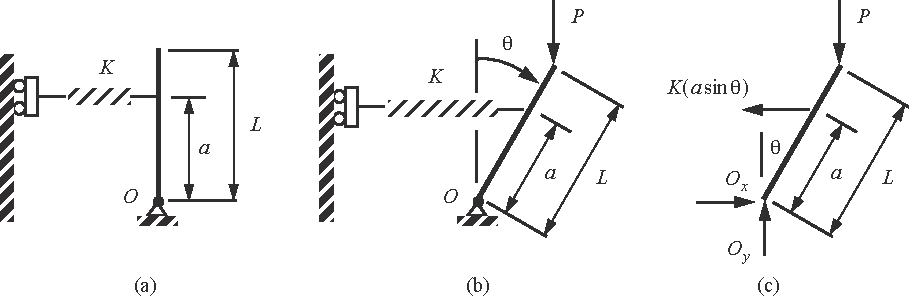
\includegraphics{Figure_10-31.pdf}
}{\caption{(a) initial configuration. (b) Deflected configuration. (c) Free body diagram.\label{fig10.31}}}}


\item[\textbf{2.}] Determine the stability of the post-buckling path for model E given by eq.~(\ref{eq10.94}) and shown in figure~\ref{fig10.28}.
\end{enumerate}
\end{exercise}

\clearemptydoublepage

\end{document} 